\chapter{神经细胞、神经回路和行为} \label{chap:chap3}



人类行为的显著多样性取决于一套精密复杂的感官接收器与大脑的连接,大脑作为一个高度灵活的神经器官,能从源源不断的感觉信号流中筛选出对个体至关重要的环境事件以及身体内部环境的变化。
大脑积极地组织感觉信息以供认知、行为、决策、审美鉴赏以及未来的参照(也就是记忆)。
同时,它也能审慎地忽略和丢弃信息,并有望明智地报告这些运作过程及其心理表现给其他的大脑。
这一切都是通过相互连接的神经细胞来实现的。


单个神经细胞或神经元是大脑的基本信号单元。 
人脑包含大量此类细胞,大约有 860 亿个神经元,这些神经元可以被划分为至少一千种不同的类型。 
然而,这些种类繁多的神经元与其说是人类行为复杂性的一个因素,不如说是它们组织成具有精确功能的解剖回路。 
事实上,大脑的一个关键组织原则是:
由于它们相连的方式不同,具有相似特性的神经细胞可以产生不同的行为。


由于神经系统的组织原则相对较少,但其功能却相当复杂,因此,可以通过关注神经系统的 5 个基本特征来深入了解神经系统如何产生行为:

1. 单个神经细胞的结构成分;

2. 神经元在自身内部和彼此之间产生信号的机制;

3. 神经细胞之间以及神经细胞与其靶标(肌肉和腺体效应器)之间的连接模式;

4. 不同互联模式与不同行为类型的关系;

5. 经验如何改变神经元及其连接。


本书的各个部分都是围绕这 5 个主要主题进行组织的。
在本章中,我们将依次介绍这些主题,概述行为的神经控制。
我们首先考虑神经元的结构和功能以及围绕和支持它们的\textit{神经胶质细胞}。
然后,我们检查单个细胞如何组织和传输信号,以及一些相互连接的神经细胞之间的信号如何产生简单的行为,即膝跳反射。
然后,我们将这些想法扩展到更复杂的行为,由更复杂和可延展的回路调节。



\section{神经系统有两类细胞}

神经系统中主要有两类细胞:\textit{神经细胞}(神经元)和\textit{胶质细胞}(神经胶质)。


\subsection{\textit{神经细胞}是神经系统的信号单位}

如图~\ref{fig:3_1}~所示,一个典型的神经元有 4 个形态学上定义的区域:\textit{细胞体}、\textit{树突}、\textit{轴突}和\textit{突触前末梢}。
正如我们将要看到的,每个区域在产生信号和与其他神经细胞通信方面都有不同的作用。


\begin{figure}[htbp]
	\centering
	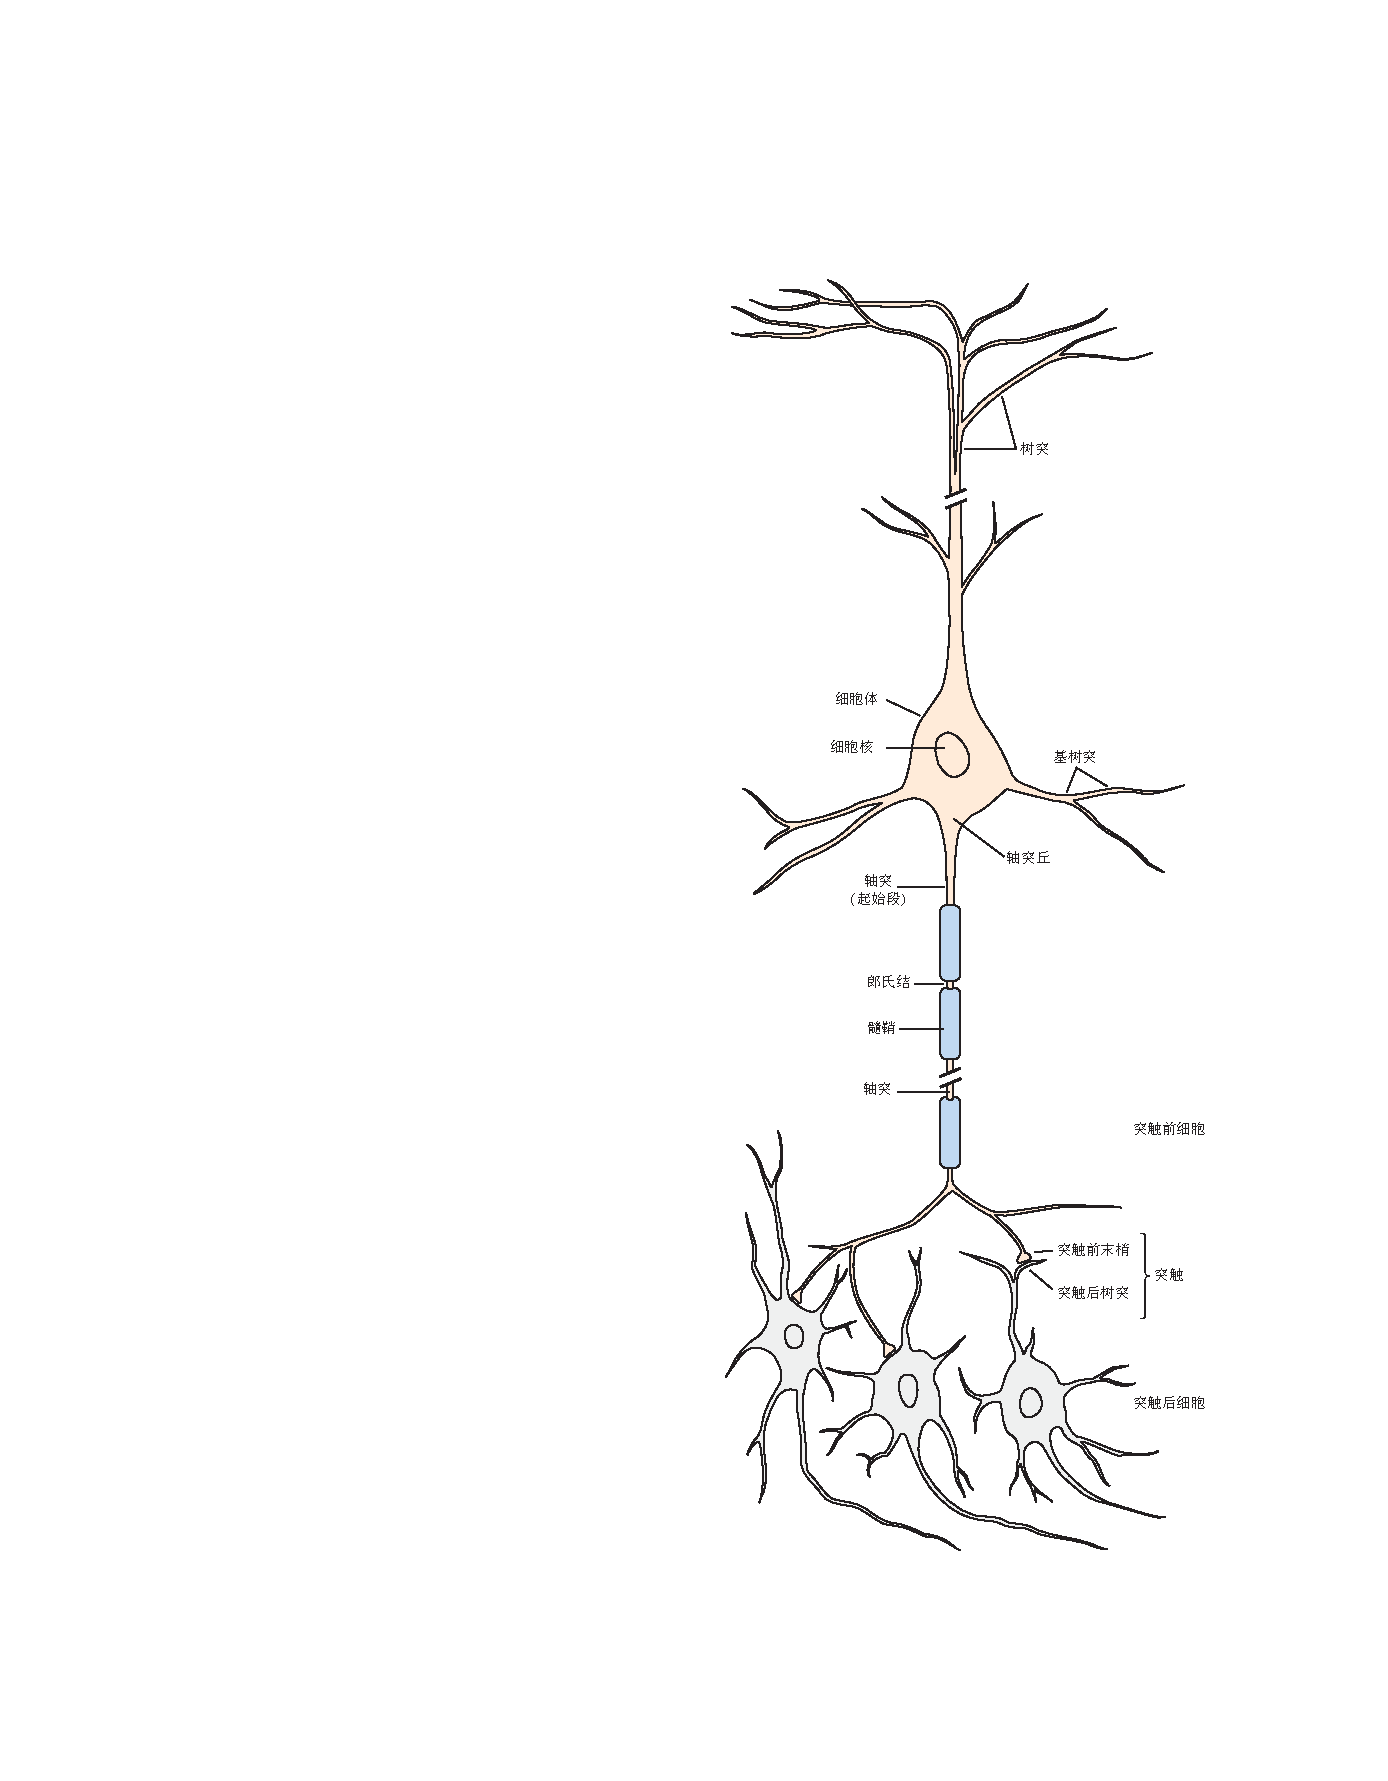
\includegraphics[width=0.6\linewidth]{chap03/fig_3_1}
	\caption{神经元的结构。 
		脊椎动物神经系统中的大多数神经元有几个共同的主要特征。
		细胞体包含细胞核,遗传信息的仓库,并产生 2 种类型的细胞过程:轴突和树突。
		轴突是神经元的传递元件;
		它们的长度差异很大,有些在体内延伸超过 1 米。 
		与细胞体的直径(50 微米或更大)相比,中枢神经系统中的大多数轴突非常细(直径在 0.2 微米和 20 微米之间)。 
		许多轴突被一层脂肪\textit{髓鞘}绝缘,该鞘在称为\textit{郎飞结}的间隙处定期中断。 
		动作电位(即细胞的传导信号)在轴突的初始部分启动并传播到突触,突触是信号从一个神经元流向另一个神经元的部位。 
		突触前神经元的轴突分支将信号传递给突触后细胞。 
		单个轴突的分支可能与多达一千个突触后神经元形成突触。 	
		顶端和基部树突与细胞体一起是神经元的输入元件,接收来自其他神经元的信号。}
	\label{fig:3_1}
\end{figure}


\textit{细胞体或胞体}是细胞的代谢中心。 
它包括含有细胞基因的细胞核和内质网,内质网是细胞核的延伸部分,细胞的蛋白质在这里合成。
细胞体会衍生出 2 种形态的结构:几个短的\textit{树突}和一个长的管状\textit{轴突}。
树突以树状方式分支,是接收来自其他神经细胞的输入信号的主要装置。 
轴突通常在分支之前从细胞体延伸一定距离,使其能够将信号传递给许多目标神经元。
轴突可以在 0.1 毫米到 1 米的距离内传输电信号。 
这些电信号或动作电位在轴突起源附近的专门触发区域启动,称为\textit{起始段},动作电位从该区域以 1 米每秒至 100 米每秒的速度沿着轴突传播而不会失败或失真。 
如图~\ref{fig:3_2}~所示,沿轴突向下传播的动作电位的振幅保持恒定在 100 毫伏,因为动作电位是一种全有或全无的脉冲,它会沿着轴突定期再生。


\begin{figure}[htbp]
	\centering
	\includegraphics[width=0.5\linewidth]{chap03/fig_3_2}
	\caption{这一历史性追踪是首次公布的动作电位细胞内记录。 
		1939 年,\textit{艾伦$\cdot$霍奇金}和\textit{安德鲁$\cdot$赫胥黎}使用充满海水的玻璃毛细管电极从乌贼巨型轴突上记录下来。
		定时脉冲(底部)间隔 2 毫秒。 
		垂直刻度表示内部电极的电位,单位为毫伏,外面的海水被视为 0 电位\cite{hodgkin1939action}。}
	\label{fig:3_2}
\end{figure}


动作电位是大脑接收、分析和传递信息的信号。 
这些信号在整个神经系统中都是高度固定的,尽管它们是由环境中影响我们身体的各种事件引发的(从光到机械接触,从气味到压力波)。
传递视觉信息的生理信号与传递气味信息的生理信号相同。
在这里,我们看到了大脑功能的一个关键原则:
动作电位传递的信息类型不是由信号的形式决定的,而是由信号在大脑中传播的通路决定。
因此,大脑分析和解释通过特定通路传输的传入电信号模式,进而创造我们的视觉、听觉、触觉、嗅觉和味觉。


为了提高传导动作电位的速度,大轴突被包裹在脂质物质髓磷脂的绝缘鞘中。
髓鞘被\textit{郎飞结}以规则的间隔中断,\textit{郎飞结}是轴突上未绝缘的点,动作电位在此再生(第~\ref{chap:chap7}~章和第~\ref{chap:chap8}~章详细讨论了髓鞘形成,第~\ref{chap:chap10}~章详细讨论了动作电位)。


在接近其末端时,轴突会分裂成细小分支,并在被称为突触的特殊通信区域与其他神经元接触。
传递信号的神经细胞称为突触前细胞;
接收信号的细胞是突触后细胞。
突触前细胞从其轴突分支的特殊扩大区域,即突触前末梢或神经末梢传输信号。
突触前细胞和突触后细胞被一个非常狭窄的空间隔开,即突触间隙。
如图~\ref{fig:3_1}~所示,大多数突触前末梢终止于突触后神经元的树突,但有部分也终止于细胞体,或者较少见的是终止于突触后细胞轴突的起点或末端。
一些突触前神经元会激发它们的突触后靶细胞;
其他突触前神经元抑制它们的靶细胞。


神经元学说(第~\ref{chap:chap1}~章)认为每个神经元都是一个具有独特形态的离散细胞,其细胞体上延伸出不同的突起,并且神经元是神经系统信号传递的基本单位。
回想起来,很难体会到科学家最初提出这个基本想法时有多难接受。
不同于其他具有简单形状且可在光学显微镜单个视野内观察到的细胞组织,神经细胞具有复杂的形状。
树突的复杂模式以及一些轴突看似无穷无尽的过程使得在这些元素之间建立关系变得极其困难。
即使在解剖学家\textit{雅各布$\cdot$施莱登}和\textit{西奥多$\cdot$施旺}于 1830 年代初期提出细胞理论(细胞是所有生命物质的结构单元的观点成为生物学的中心教条)之后,大多数解剖学家仍然没有接受细胞理论适用于大脑,他们认为大脑是一个连续、网状的薄细过程构成的复杂体系。


神经元的连贯结构直到 19 世纪后期才变得清晰,当\textit{拉蒙$\cdot$卡哈尔}开始使用高尔基体引入的银染法时。
这种方法至今仍在使用,它有 2 个优点。
首先,银溶液以一种尚未完全理解的随机方式,仅染色大脑特定区域中约 1\% 的细胞,这使得研究者能够单独地从邻近细胞中观察单一神经元。
其次,被染色的神经元呈现出完整的形态,包括细胞体、轴突和全部的树突分支。
染色表明神经元之间没有细胞质连续性,\textit{卡哈尔}预言性地正确地得出结论,即使在 2 个细胞之间的突触处也没有连续性。


\textit{拉蒙$\cdot$卡哈尔}不仅将高尔基染色法应用于人类胚胎神经系统,还将其扩展到了多种动物的胚胎神经系统。 
通过观察几乎整个神经系统中神经元的结构,他可以描述神经细胞的类别并绘制出许多神经细胞之间的精确联系。
通过这种方式,除了神经元学说之外,\textit{拉蒙$\cdot$卡哈尔}还推导出了另外 2 个神经组织原理,这 2 个原理在研究神经系统的交流方面特别有价值。


% 传播方向的极化(偏向于一边)?
其中第一个是\textit{动态极化}原理,它指出神经细胞内的电信号仅沿一个方向流动:
从神经元的突触后部位(通常是树突和细胞体)流向轴突的触发区域。
在那里,动作电位沿着轴突的整个长度传播到其末端。
在迄今为止研究的大多数神经元中,电信号实际上沿着轴突单向传播。


\textit{拉蒙$\cdot$卡哈尔}提出的第二个原则(即\textit{连接特异性})指出在神经网络形成过程中,神经细胞并非随机地彼此连接,而是在特定的接触点与某些特定的突触后靶细胞建立特定的连接关系,而非与其他细胞随意连接。
\textit{动态极化}原理和\textit{连接特异性}原理是现代细胞连接主义研究大脑方法的基础。


\textit{拉蒙$\cdot$卡哈尔}也是最早意识到区分不同类型神经元的最主要特征是其形态,特别是细胞体产生突起过程的数量。 
因此,神经元分为 3 大类:单极神经元、双极神经元和多极神经元。


单极神经元是最简单的,因为它们只有一个主要突起,通常会产生许多分支。
如图~\ref{fig:3_3}A~所示,一个分支作为轴突,其他分支充当接收结构。
这些细胞在无脊椎动物的神经系统中占主导地位;
在脊椎动物中,它们出现在\textit{自主神经系统}中。


\begin{figure}[htbp]
	\centering
	\includegraphics[width=0.95\linewidth]{chap03/fig_3_3}
	\caption{根据源自细胞体的过程的数量,神经元分为单极、双极或多极。 
		A. 单极细胞有一个从细胞体发出的单一突起。
		不同的部分作为接受表面或释放末梢。
		单极细胞是无脊椎动物神经系统的特征。 
		B. 双极细胞有 2 种功能特化的突起。
		树突接收电信号,轴突将信号传递给其他细胞。
		C. 伪单极细胞是双极细胞的变体,负责将体感信息传递到脊髓。
		在发育过程中,胚胎期双极细胞原有的 2 个突起融合,形成一个从细胞主体出发的单一过程,该过程具有 2 个功能不同的部分。
		 2 个部分都起轴突的作用;
		一个延伸到外周皮肤或肌肉,另一个延伸到中枢脊髓\cite{ross2006histology}。
		D. 多极细胞具有单个轴突和许多树突。 
		它们是哺乳动物神经系统中最常见的神经元类型。 
		以下 3 个例子说明了这些细胞的巨大多样性。
		脊髓运动神经元支配骨骼肌纤维。
		锥体细胞具有大致呈三角形的细胞体;
		树突从顶点(顶端树突)和基部(基底树突)出现。 
		锥体细胞存在于海马体和整个大脑皮层中。 
	小脑的浦肯野细胞以其丰富且广泛分布的树突网络为特点,能容纳数量庞大的突触输入\cite{ross2006histology}。}
	\label{fig:3_3}
\end{figure}


\textit{双极神经元}有一个椭圆形的体细胞,它产生 2 个不同的突起结构:
如图~\ref{fig:3_3}B~所示,一个负责接收来自其他神经元信号的树突结构和一个将信息传向中枢神经系统的轴突。
许多感觉细胞是双极神经元,包括\textit{视网膜双极细胞}和鼻子的嗅觉上皮细胞。
将触觉、压力和疼痛信号传递至脊髓的受体神经元最初也表现为双极细胞,但随后 2 个细胞突起会融合成一个连续的单一结构,从细胞体的一个点处发出,同时,原本的树突获得了使其成为轴突的特殊化结构。
如图~\ref{fig:3_3}C~所示,在这些所谓的\textit{假单极细胞}中,一个轴突将信息从皮肤、关节和肌肉中的感觉受体传递到细胞体,而另一个轴突将此感觉信息传递到脊髓。


如图~\ref{fig:3_3}D~所示,\textit{多极神经元}在脊椎动物的神经系统中占主导地位。 
它们通常有一个单一的轴突和多个从细胞体周围不同位置发出的树突结构。
多极细胞的形状差异极大,特别是在轴突长度及其树突分支的程度、尺寸和复杂性方面。 
通常,树突分支的程度与其它神经元与其形成的突触联系数量相关联。 
一个树突数量相对较少的脊髓运动神经元接受大约 1 万个接触,其中 1 千个在细胞体上,9 千个在树突上。
在小脑的\textit{浦肯野细胞}中,树突树更大更茂密,接受多达一百万次接触!


神经细胞也分为 3 个主要功能类别:
感觉神经元、运动神经元和中间神经元。 
\textit{感觉神经元}感觉神经元负责将身体周边传感器的信息传递到神经系统中,以便进行感知和运动协调。
一些\textit{初级感觉神经元}称为\textit{传入神经元},这 2 个术语可以互换使用。
术语\textit{传入}(传向中枢神经系统)适用于从外围到达中枢神经系统的所有信息,无论该信息是否导致感觉。
术语\textit{感觉}是指那些将信息从感觉上皮细胞、关节感觉受体或肌肉传递到中枢神经系统的传入神经元,但该概念已扩展到包括初级和次级皮质区域中对感觉特征变化作出反应的神经元,例如物体在空间中的位移、声音频率的变化或头部的角旋转(通过耳朵中的前庭器官),甚至像面部这样复杂的东西。


\textit{传出}一词适用于从中枢神经系统向运动器官传递的所有信息,无论这些信息是否导致行动。
\textit{运动神经元}将命令从大脑或脊髓传递到肌肉和腺体(传出信息)。 
运动神经元(或运动神经元)的传统定义是激发肌肉活动的神经元,但现在运动神经元的范畴还包括那些不直接支配肌肉但却间接指挥动作的其他神经元。
无论是运动神经元还是感觉神经元,它们共同的特点是对神经系统之外事物的时间保真度。
它们的活动与外部刺激的变化以及身体肌肉施加的动力动态保持一致。	
感觉神经元为大脑提供数据,而运动神经元将观念转化为实践。 
它们共同构成了我们与世界的连接。


\textit{中间神经元}包含最多的功能类别,并细分为两类:\textit{中继中间神经元}和\textit{局部中间神经元}。
中继中间神经元或投射中间神经元具有较长轴突,可在相当长的距离内将信号从一个大脑区域传送到另一个大脑区域。
局部中间神经元的轴突较短,因为它们与局部回路中附近的神经元形成连接。
由于几乎每个神经元都可以被视为中间神经元,因此这一术语常用来区别以下 2 种神经元:一种是在局部回路内投射到另一个神经元的神经元,另一种则是投射到单独神经结构的神经元。
该术语有时也用作抑制性神经元的简写,特别是在皮层回路的研究中,但为了明确表述,应在适当的时候使用\textit{抑制性中间神经元}术语。


每个功能分类可以进一步细分。 
感觉系统中间神经元可以根据它们响应的感觉刺激的类型进行分类; 
这些初步分类可以根据位置、密度、大小以及基因表达模式进一步细分。
事实上,由于\textit{信使核糖核酸}序列分析的进步使得对单个神经元进行分子表型分析成为可能,我们对神经元复杂性的认识正在迅速发展。 
如图~\ref{fig:3_4}~所示,此类分析最近揭示了神经元类型的多样性比以前认为的要大得多。


\begin{figure}[htbp]
	\centering
	\includegraphics[width=1.0\linewidth]{chap03/fig_3_4}
	\caption{感觉神经元可以细分为功能不同的组。
		例如,至少有 13 种类型的视网膜神经节细胞是根据它们的树突的大小和形状以及它们接收输入信号的视网膜深度来区分的。
		\textit{内网层}包含视网膜中间神经元(双极细胞和无长突细胞)和神经节细胞之间的连接\cite{dacey2003fireworks}。}
	\label{fig:3_4}
\end{figure}



\subsection{\textit{胶质细胞}支撑神经细胞}
\textit{胶质细胞}的数量远远超过神经元,在脊椎动物中枢神经系统中,胶质细胞的数量是神经元的 2 到 10 倍。
尽管这些细胞的名称源自希腊语中的\textit{胶水},但实际上胶质细胞并不普遍起着粘合神经细胞的作用。
相反,它们围绕着神经元的细胞体、轴突和树突。
胶质细胞在形态上不同于神经元,
它们不形成树突和轴突。


胶质细胞在功能上也有所不同。
尽管它们来自相同的胚胎前体细胞,但其膜特性与神经元并不相同,因此不具备电兴奋性。
因此,它们并不直接参与神经元的电信号传递这一功能。
然而,它们在帮助电信号快速沿神经元轴突传递方面发挥着作用,并且似乎在早期发育过程中指导神经连接以及通过学习形成新的或改变的神经元间连接的稳定性上扮演着重要角色。
在过去的 10 年中,人们对胶质细胞的多种功能的兴趣有所增加,对其特性的认知也从支持细胞转变为神经元的功能性伙伴(第~\ref{chap:chap7}~章)。



\section{每个神经细胞都是调节特定行为的回路的一部分}

每种行为都由一组特定的相互连接的神经元介导,而每一个神经元的行为功能都取决于它与其他神经元的联系。
一个简单的膝跳反射行为将说明这一点。 
当身体短暂的不平衡拉伸腿部股四头肌伸肌时,反射开始。
这种拉伸会产生传送给运动神经元的感觉信息,而运动神经元又会向伸肌发出收缩命令,从而恢复平衡。


这个反射在临床上被用于检测神经的完整性以及脊髓对反射幅度(或增益)的控制情况。 
潜在的机制很重要,因为它可以维持股四头肌的正常张力,并防止我们的膝盖在站立或行走时屈曲。 
股四头肌是一块伸展小腿的肌肉,其肌腱通过髌骨(膝盖骨)的肌腱附着在胫骨上。
轻敲髌骨正下方的肌腱可以拉伸股四头肌。 
这种拉伸会启动股四头肌的反射性收缩,产生我们熟悉的膝跳。 
如图~\ref{fig:3_5}~所示,通过增加选定肌肉群的张力,牵张反射改变腿的位置,突然向外伸展。

\begin{figure}[htbp]
	\centering
	\includegraphics[width=0.68\linewidth]{chap03/fig_3_5}
	\caption{膝跳反射由感觉神经元和运动神经元组成的一个简单回路所控制。
		用叩诊锤轻叩膝盖骨会拉动股四头肌的肌腱,股四头肌是拉伸小腿的肌肉。
		当肌肉因肌腱的牵拉而伸展时,有关肌肉变化的信息会通过感觉神经元传送到中枢神经系统。
		在脊髓中,感觉神经元与伸肌运动神经元形成兴奋性突触,这些运动神经元会使受到牵拉的股四头肌收缩。 
		感觉神经元通过中间神经元间接作用于拮抗肌(腿筋的屈肌运动神经元),抑制其收缩。
		这些作用结合起来产生膝跳反射行为。 
		在图中,每个伸肌和屈肌运动神经元代表许多细胞群。}
	\label{fig:3_5}
\end{figure}


参与膝跳反射的感觉神经元细胞体聚集在背根神经节的脊髓附近。
它们是假单极细胞;
每个细胞轴突的一个分支延伸到周围的股四头肌,而另一支则向中央方向进入脊髓内部。
延伸至股四头肌的那一分支与感受肌肉伸展敏感性的受体(肌梭)接触,并在肌肉被拉伸时被激活。
进入脊髓并与之形成兴奋性联系的那一分支与控制股四头肌收缩的运动神经元相连。
如图~\ref{fig:3_5}~所示,该分支还联系抑制控制相对屈肌的运动神经元的局部中间神经元。 
尽管这些局部中间神经元并未直接参与到伸展反射本身的发生过程中,但它们通过协调对抗肌群的活动来提高反射动作的稳定性。
因此,产生牵张反射的电信号携带 4 种信息:

1. 感觉信息从肌肉传递到中枢神经系统(脊髓)。

2. 来自中枢神经系统的运动命令被发送到进行膝跳的肌肉。

3. 向拮抗肌的运动神经元发出抑制指令。

4. 与膝跳有关的局部神经元活动的信息被发送到中枢神经系统的更高中枢,允许大脑同时或依次协调不同的行为。


此外,大脑还会根据情境实施对膝跳反射的依赖性控制以调整其强度。
例如,当我们跑步时,腿筋会弯曲膝盖,从而拉伸股四头肌。
大脑和脊髓抑制牵张反射,使股四头肌放松。
当这些下行通路被破坏时,就像在中风病例那样,反射被放大并且关节变得僵硬。


仅仅拉伸一块肌肉(股四头肌),就会激活数百个感觉神经元,每个神经元与 45 到 50 个运动神经元直接接触。
如图~\ref{fig:3_6}A~所示,这种一个神经元激活多个目标细胞的连接模式称为分散。 
它在神经系统的输入阶段尤为常见;
通过将其信号分配给许多靶细胞,单个神经元可以发挥广泛而多样的影响。 
相反,在膝跳反射回路中,单个运动细胞会接受来自大约 130 个感觉细胞的大约 200 至 450 个输入联系。
如图~\ref{fig:3_6}B~所示,这种连接模式称为\textit{汇聚}。
它在神经系统的输出阶段很常见;
一个接收来自多个感觉神经元信息的目标运动细胞能够整合多种来源的信息。
每个感觉神经元输入产生相对较弱的兴奋,因此\textit{汇聚}也有助于确保只有当足够数量的感觉神经元一起被激活时,运动神经元才会被激活。


\begin{figure}[htbp]
	\centering
	\includegraphics[width=0.5\linewidth]{chap03/fig_3_6}
	\caption{发散和汇聚的神经元连接是大脑的一个关键组织特征。
		A. 在感觉系统中,通常每个受体神经元会与多个代表第二级处理阶段的神经元相连。 
		在随后的处理阶段,传入的连接会进一步发散。 
		这种结构使得来自单一感受部位的感觉信息能够在脊髓和大脑中得到更广泛的分布。
		B. 相比之下,运动神经元是逐渐融合连接的目标。 
		在这种结构安排下,需要来自多个突触前细胞的输入才能激活运动神经元。}
	\label{fig:3_6}
\end{figure}


% A stretch reflex such as the knee-jerk reflex
诸如膝跳反射这样的牵张反射是一种由两类神经元在兴奋性突触处连接产生的简单行为。
但并非大脑中的所有重要信号都是兴奋性的。 
许多神经元会产生抑制信号,从而降低神经元放电的可能性。 
即使在简单的膝跳反射中,感觉神经元也会同时形成兴奋性连接和抑制性连接。
在腿部伸肌中的兴奋性连接会导致这些肌肉收缩,而与抑制性中间神经元的连接则阻止拮抗肌(屈肌)收缩。 
如图~\ref{fig:3_7}A~所示,回路的这个特性是前馈抑制的一个例子。 
在膝跳反射中,前馈抑制意味着感觉神经元的信息不仅触发了伸肌的收缩,还通过中间神经元提前抑制了屈肌的收缩,从而保证了膝关节的协调运动。


\begin{figure}[htbp]
	\centering
	\includegraphics[width=0.62\linewidth]{chap03/fig_3_7}
	\caption{抑制性中间神经元可以产生前馈抑制或反馈抑制。
		A. 前馈抑制通过抑制调节相反作用通路的活性来增强活性通路的效果。
		前馈抑制在单突触反射系统中很常见。 
		例如,如图~\ref{fig:3_5}~所示,在膝跳反射回路中,来自伸肌的传入神经元不仅会刺激伸肌运动神经元,还会刺激抑制性中间神经元,这些中间神经元会阻止支配拮抗肌(屈肌)的运动细胞放电。
		B. 反馈抑制是一种自我调节机制。
		在这种机制中,伸肌运动神经元作用于抑制性中间神经元,而这些中间神经元反过来又作用于原先的伸肌运动神经元,从而降低它们的放电概率。
		其作用是抑制受刺激通路内的活动并防止其超过某个临界水平。}
	\label{fig:3_7}
\end{figure}


一些回路提供反馈抑制。 
例如,一个运动神经元可能既与一块肌肉形成兴奋性连接,又与一个抑制性中间神经元形成连接,而这个抑制性中间神经元自身也会与运动神经元相连。
如图~\ref{fig:3_7}B~所示,当运动神经元兴奋并激发抑制性中间神经元时,中间神经元能够限制运动神经元刺激肌肉的能力力。
当我们在后面的章节中研究更复杂的行为时,我们会遇到许多前馈抑制和反馈抑制的例子。


\section{信号在所有神经细胞中的组织方式相同}
为了产生一种行为(例如牵张反射),参与其中的每个感觉神经细胞和运动神经细胞都必须按顺序在其内部不同位置生成 4 种不同的信号。
尽管细胞大小和形状、传递生物化学物质或行为功能各不相同,但几乎所有神经元都可以用一个模型神经元来描述,该模型神经元具有产生 4 种类型信号的 4 个功能组件:
如图~\ref{fig:3_8}~所示,一个用于产生分级输入信号的接收组件,一个产生触发信号的总和或整合组件,一个产生全有或全无传导信号的长程传导组件,以及产生输出信号到下一个神经元或肌肉或腺体细胞的突触组件。


\begin{figure}[htbp]
	\centering
	\includegraphics[width=1.0\linewidth]{chap03/fig_3_8}
	\caption{大多数神经元有 4 个功能区域,在这些区域中会生成不同类型的信号。
		因此,大多数神经元的功能组织(无论类型如何)都可以用模型神经元示意性地表示。
		该模型神经元是\textit{拉蒙$\cdot$卡哈尔}动态极化原理的生理表达。 
		输入信号、综合信号和传导信号都是电信号,对细胞来说是不可或缺的,而输出信号是由细胞射入到突触间隙的化学物质。
		并非所有神经元都具有所有这些特征。 
		例如,一些局部中间神经元就缺乏长程传导组件。}
	\label{fig:3_8}
\end{figure}


神经元产生的不同类型信号在一定程度上由细胞膜的电学特性决定。
任何细胞(包括神经元)在静息状态下,细胞膜两侧都会保持一定的电位差。
这称为静息膜电位。 
在典型的静息神经元中,细胞内侧的电压比细胞外侧的电压大约低65毫伏。
因为膜外电压被定义为 0,所以我们说静息膜电位为 –65 毫伏。
不同神经细胞的静息电位范围为 –40 毫伏至 –80 毫伏; 
在肌肉细胞中(它更大)约为 –90 毫伏。
正如第~\ref{chap:chap9}~章中详细描述的那样,静息膜电位由 2 个因素造成:
带电离子的不均匀分布(特别是带正电的~\ce{Na+} 和~\ce{K+}),以及膜的选择性渗透性。


细胞膜两侧阳离子不均衡分布的维持主要依赖于 2 种机制。
细胞内~\ce{Na+} 和~\ce{K+} 浓度主要由膜蛋白控制,膜蛋白主动将~\ce{Na+} 泵出细胞并将~\ce{K+} 泵回细胞内。
这个~\ce{Na+}-\ce{K+} 泵,我们将在第~\ref{chap:chap9}~章中详细了解,它使细胞内的~\ce{Na+} 浓度保持在较低水平(约为细胞外浓度的 1/10),并使~\ce{K+} 浓度保持在较高水平(约为细胞外浓度的 20 倍)。
\ce{Na+} 和~\ce{K+} 的细胞外浓度由肾脏和星形胶质细胞(也称为星形胶质细胞)维持。


除此之外,原本无法穿透的细胞膜包含形成离子通道的蛋白质。
细胞静止时活跃的通道对~\ce{K+} 的渗透性很高,但对~\ce{Na+} 的渗透性要低得多。
\ce{K+} 往往会沿着离子的浓度梯度从这些开放通道中泄漏出来。
当~\ce{K+} 离开细胞时,它们会在膜的内表面留下一团未中和的负电荷,因此膜内的净电荷比膜外的负电荷更多。
在这种情况下,相对于神经元外部,膜电位通常保持在 –65 毫伏左右,据说神经元处于静止状态。


当细胞开始吸收细胞外浓度较高的~\ce{Na+}(或~\ce{Ca^2+})时,静息状态就会受到干扰。
这些带正电的离子向内运动(内向电流)部分地中和了细胞内部的负电压。 
我们将在下面详细介绍这些事件。 
然而,接下来发生的事情对于理解神经元为何适合用于信息传递至关重要。


当细胞(如神经细胞和肌肉细胞)的膜电位能够迅速且显著改变时,我们称这类细胞为可兴奋细胞。 
在许多神经元中,膜电位 10 毫伏的变化(从 –65 毫伏到 –55 毫伏)使膜对~\ce{Na+} 的渗透性比对~\ce{K+} 的渗透性强得多。
由此产生的~\ce{Na+} 流入进一步中和了细胞内的负电荷,导致对~\ce{Na+} 的渗透性更高。
结果是膜电位发生短暂的爆炸性变化,变为 +40 毫伏,即动作电位。 
此电位会沿着细胞轴突积极传导至轴突末梢,在那里引发与突触后神经元或肌肉细胞复杂的化学相互作用。
由于动作电位是主动传播的,因此其振幅在到达轴突末梢时不会减小。
动作电位通常持续约 1 毫秒,之后膜电位会恢复至静息状态,恢复正常的电荷分离状态,并重新呈现对~\ce{K+} 的渗透性高于对~\ce{Na+} 的渗透性。


静息电位和动作电位的潜在机制在第~\ref{chap:chap9}~章和第~\ref{chap:chap10}~章中详细讨论。
除了动作电位代表的长距离信号外,神经细胞还产生局部信号(受体电位和突触电位位),这些信号不被积极传导,通常在几毫米范围内就会衰减(见下一节)。


引起长距离信号和局部信号的膜电位变化既可以是从静息电位的下降,也可以是上升。
也就是说,静息膜电位是所有信号发生的基准线。 
膜电位的下降(称为去极化)增强了细胞产生动作电位的能力,因此具有兴奋性。 
相反,膜电位的上升,称为超极化,使细胞更难产生动作电位,因此具有抑制作用。


\subsection{输入组件产生分级本地信号}
在大多数处于静息状态的神经元中,电流不会从细胞的一部分流向另一部分,所以静息电位在整个细胞中是一致的。 
在感觉神经元中,电流通常由物理刺激启动,物理刺激会激活神经元接受表面的特殊受体蛋白。 
在我们膝跳反射的例子中,肌肉的拉伸会激活特定的离子通道,这些离子通道会响应感觉神经元膜的拉伸而打开,我们将在第~\ref{chap:chap18}~章中了解到。
当细胞被拉伸时,这些通道的打开允许~\ce{Na+} 快速流入感觉细胞。
这种离子电流改变膜电位,产生称为受体电位的局部信号。


如图~\ref{fig:3_9}A~所示,受体电位的幅度和持续时间取决于肌肉拉伸的强度:拉伸越大或持续时间越长,由此产生的受体电位越大或持续时间越长。
也就是说,受体电位是分级的,这与\textit{全有或全无}动作电位不同。
大多数受体电位是去极化的(兴奋性的);
在视网膜中发现超极化(抑制性)受体电位。


\begin{figure}[htbp]
	\centering
	\includegraphics[width=1.0\linewidth]{chap03/fig_3_9}
	\caption{神经元的 4 个信号成分中的每一个都会产生一个特征信号。
		该图显示了通过肌肉拉伸激活的感觉神经元,神经元通过专门的受体(肌梭)感知。 
		A. 输入信号(称为受体电位)在振幅和持续时间上分级,与刺激的振幅和持续时间成正比。 
		B. \textit{触发区}总结了受体电位产生的去极化。
		只有当受体电位超过某个电压阈值时才会产生动作电位。
		一旦超过这个阈值,受体电位幅度的任何进一步增加只能增加动作电位产生的频率,因为动作电位具有恒定的幅度。
		受体电位的持续时间决定了动作电位序列的持续时间。
		因此,受体电位的分级振幅和持续时间被转化为触发区产生的动作电位中的频率编码。
		产生的所有动作电位都忠实地沿着轴突传播。
		C. 动作电位是全有或全无。
		因为所有动作电位都具有相似的幅度和持续时间,所以放电的频率和持续时间编码了信号所携带的信息。
		D. 当动作电位到达突触末梢时,它会启动神经递质的释放,即用作输出信号的化学物质。
		突触前细胞中动作电位的频率决定了细胞释放多少神经递质。}
	\label{fig:3_9}
\end{figure}


受体电位是对神经系统中拉伸首次进行编码的表现形式示。
然而,由于这种去极化从拉伸受体被动传播,它不会传播很远。
如果轴突的直径较大,则距离较长,如果直径较小,则距离较短。
此外,如果电流可以轻松通过膜,则距离会更短,如果膜被髓磷脂绝缘,则距离会更长。
因此,来自拉伸受体的受体电位仅移动 1 至 2 毫米。
事实上,就在 1 毫米远的地方,信号的幅度仅为产生位置的 1/3 左右。
为了成功地传送到脊髓,局部信号必须被放大,即它必须产生动作电位。
在膝跳反射中,如果感觉神经元中的受体电位到达轴突的第一个郎飞结并且足够大,它将触发一个动作电位(图~\ref{fig:3_9}B),然后这个动作电位将无损地传播到脊髓中的轴突末梢(图~\ref{fig:3_9}C)。
在感觉神经元和运动神经元之间的突触处,动作电位会产生一系列事件,这些事件会导致运动神经元的输入信号。


如图~\ref{fig:3_9}D~所示,在膝跳反射中,感觉神经元突触前末梢的动作电位会引发一种化学物质(即神经递质),释放到突触间隙中。
神经递质在穿越突触间隙后,会与运动神经元突触后膜上的受体蛋白质结合,从而直接或间接地开启离子通道。
随后的电流流动会短暂地改变运动细胞的膜电位,这种变化称为突触电位。


与受体电位一样,突触电位也是分级的; 
其振幅取决于释放了多少神经递质。 
在同一细胞中,根据激活的是何种类型的受体分子,突触电位可以是去极化的,也可以是超极化的。 
突触电位和如受体电位一样,被动传播。 
因此,除非信号传播到轴突起始段并足以引发动作电位,否则电位的变化将仅限于局部。
一些树突并非完全被动,而是包含着能够增强突触电位的特殊结构,从而提高其产生动作电位的有效性(第~\ref{chap:chap13}~章)。 
表~\ref{tab:3_1}~总结了受体和突触电位的特征。


\begin{table}[htbp]
	\caption{局部(被动)和传播信号的比较} \label{tab:3_1} \centering
	\begin{tabular}{llllll}
		\toprule
		信号类型 & 振幅(毫伏) & 持续时间 & 总和 & 信号效应 & 传播类型\\
		\midrule
		\makecell{局部被动信号\\受体电位} & 小(0.1–10) & 短暂(5-100毫秒) & 分级 & 超级化或去极化 & 被动 \\
		\midrule
		突触电位 & 由短到长 & 短暂(5-100毫秒) & 分级 & 超级化或去极化 & 被动 \\
		\makecell{传播(激活)的信号\\动作电位} & 大(70–110) & 短暂(1-10毫秒) & 全有或全无 & 
		去极化 & 主动 \\
		\bottomrule
	\end{tabular}
\end{table}


\subsection{触发区决定产生动作电位}
谢林顿首先指出,神经系统的功能是权衡不同类型信息的后果,然后决定适当的反应。 
神经系统这种整合功能在神经元触发区,即轴突的起始段的事件中表现得尤为明显。


动作电位是由~\ce{Na+} 通过细胞膜中的通道突然流入而产生的,这些通道响应于膜电位的变化而打开和关闭。
当输入信号(受体电位或突触电位)使膜区域去极化时,膜电位的局部变化会打开局部~\ce{Na+} 通道,使~\ce{Na+} 沿着其浓度梯度从~\ce{Na+} 浓度高的细胞外向细胞内低浓度处流动。


由于轴突起始段具有最高的电压敏感性~\ce{Na+} 通道,因此产生动作电位的阈值最低沿细胞膜被动传播的输入信号在此处比在细胞其他部位更可能引发动作电位。
因此,这部分轴突被称为触发区。
所有受体(或突触)电位的活动被汇总,如果输入信号的总和达到阈值,神经元就会产生动作电位。


\subsection{导电成分传播全有或全无动作电位}
动作电位是全有或全无:
低于阈值的刺激不会产生信号,但高于阈值的刺激都会产生相同幅度的信号。
无论刺激强度或持续时间的变化如何,每个动作电位的幅度和持续时间几乎都是恒定的,这适用于沿着有髓轴突的朗飞节点处的每个再生动作电位。
此外,与被动传播并随距离增加而幅度减小的受体电位和突触后电位不同,正如我们所见,动作电位在沿着轴突到达其目标(距离可达 1 米)时不会衰减。 
因为它是周期性再生的。
这种传导信号可以以高达 100 米每秒的速度传播。
事实上,动作电位的显著特征是它们是高度标准化的,从一个神经细胞到另一个神经细胞的变化很小(在某些情况下很重要)。
\textit{埃德加$\cdot$阿德里安}在 20世纪20年代证明了这一特征,他是最早在细胞水平上研究神经系统的人之一。
如图~\ref{fig:3_2}~所示,\textit{阿德里安}发现所有动作电位都具有相似的形状或波形。
由感觉轴突带入神经系统的动作电位与由运动轴突从神经系统带入肌肉的动作电位通常无法区分。


如图~\ref{fig:3_9}C~所示,传导信号只有 2 个特征传达信息:动作电位的数量和它们之间的时间间隔。
正如\textit{阿德里安}在 1928 年总结他对感觉纤维的研究时所说:“所有的冲动都非常相似,无论信息是注定要引起光感、触感还是痛感;
如果它们挤在一起,感觉就会强烈,如果它们相距很远,感觉就会相应地微弱。” 
因此,决定感觉强度或运动速度的是动作电位的频率。
同样,感觉或运动持续的时间由动作电位产生的时间跨度决定。


除了动作电位的频率,动作电位的模式也传达了重要的信息。
例如,一些神经元在没有刺激的情况下会自发活跃。
一些自发活跃的神经细胞(跳动的神经元)有规律地激发动作电位;
其他人(爆发的神经元)在短暂的动作电位爆发中激活。
这些不同的细胞对相同的兴奋性突触输入有不同的反应。
兴奋性突触电位可能会在非自发活动的细胞中引发一个或多个动作电位,而同样的输入对于自发活动的细胞来说只会简单地增加现有的发放频率。


当输入信号具有抑制性时,会出现更显著的差异。
在静默的细胞中,抑制性输入的信息价值很小。 
相比之下,在自发活跃的细胞中,抑制可以起到强大的塑造作用。
通过在持续活动期间建立沉默期,抑制能够产生一种原本不存在的、交替的放电和静默的复杂模式。
这种放电模式中的细微差别可能对神经元间信息传递的功能后果具有重要意义。
神经网络的数学模型研究者试图阐述神经编码方式,其中信息不仅由动作电位的频率携带,还由每个动作电位确切的时间安排,即放电模式的精细结构来承载。


如果信号是模式化的,仅反映刺激的基本属性,那么它们如何携带复杂行为所需的丰富信息呢?
如何将包含蜜蜂视觉信息的信息与包含蜜蜂蜇伤疼痛信息的信息区分开来?
这些感觉信号是如何与传达自主运动的运动信号区分开来的呢?
答案既简单又直接,它是神经系统最重要的组织原则之一:
相互连接的神经元形成解剖学和功能上不同的通路(标记线)正是这些连接神经元的通路,这些标记线,而不是单个神经元都传达信息。 
视网膜中对光响应的感受细胞激活的神经通路与皮肤中对触摸响应的感受细胞激活的通路是完全不同的。


\subsection{输出组件释放神经递质}

当动作电位到达神经元的末端时,它会刺激细胞释放化学物质。
这些物质称为神经递质,可以是有机小分子,例如L-谷氨酸和乙酰胆碱,也可以是肽,例如 P 物质或\textit{黄体生成素-释放激素}。


神经递质分子储存在称为突触囊泡的亚细胞器官中,这些囊泡在轴突末梢的特殊释放位点,称为活性区。
为了将递质物质喷射到突触间隙(即突触前和突触后细胞之间的细胞外空间),囊泡会移动至并与神经元的细胞膜融合,然后通过一个称为胞吐的过程爆裂开来释放递质。
第~\ref{chap:chap14}~章和第~\ref{chap:chap15}~章描述了神经递质释放的分子机制。


释放的神经递质分子是神经元的输出信号。 
因此,如图~\ref{fig:3_9}C、D~所示,根据释放的递质量来分级输出信号,而这取决于到达突触前末梢的动作电位的数量和频率。
释放后,递质分子扩散穿过突触间隙并与突触后神经元上的受体结合。
这种结合导致突触后细胞产生突触电位。
突触电位具有兴奋性或抑制性效应取决于突触后细胞中受体的类型,而不是特定的化学神经递质类型。
相同的递质物质在不同的受体上可能有不同的作用。



\subsection{牵张反射通路说明了神经信号从感觉到运动的转变}

正如我们所见,当信号从神经元的一个组成部分移动到另一个组成部分或在神经元之间移动时,信号的特性会发生变化。
如图~\ref{fig:3_10}A~所示,在牵张反射中,当肌肉被拉伸时,刺激的幅度和持续时间反映在感觉神经元中产生的受体电位的幅度和持续时间中。
如果受体电位超过该细胞中动作电位的阈值,则分级信号会在触发区转换为动作电位。
尽管单个动作电位都是全有或全无的信号,但受体电位超过阈值越多,去极化程度就越大,因而轴突中的动作电位频率也就越高。
输入信号的持续时间也决定了动作电位序列的持续时间。


\begin{figure}[htbp]
	\centering
	\includegraphics[width=1.0\linewidth]{chap03/fig_3_10}
	\caption{产生反射动作的信号序列。
		A. 肌肉的拉伸会在专门的受体(肌梭)中产生受体电位。 
		受体电位的幅度与拉伸的强度成正比。 
		这个电位被动地传播到第一个郎飞氏结处的整合区或触发区。
		如果受体电位足够大,它就会触发一个动作电位,随后该动作电位沿着轴突主动且不变地传播到轴突末梢。
		在末端的特定位点,动作电位导致化学神经递质的释放,这是输出信号。
		递质扩散穿过轴突末梢和支配拉伸肌肉的目标运动神经元之间的突触间隙;
		然后它与运动神经元外膜上的受体分子结合。
		B. 这种相互作用启动了一个突触电位,该电位被动地传播到运动神经元轴突的触发区,在那里它启动一个动作电位,该动作电位再主动传播到运动神经元轴突的末梢。
		在轴突末梢,动作电位导致在靠近肌肉纤维的位置释放神经递质。
		C. 神经递质结合肌纤维上的受体,产生突触电位。
		突触电位触发肌肉中的动作电位,从而引起收缩。}
	\label{fig:3_10}
\end{figure}


由放电频率和持续时间编码的信息忠实地沿着轴突传递到其末端,在那里,动作电位的发放决定了释放的递质量。 
这些信号阶段在运动神经元(图~\ref{fig:3_10}B)和肌肉(图~\ref{fig:3_10}C)中有对应的阶段。


\section{神经细胞在分子水平上的差异最大}
我们概述的神经元信号传导模型是一个简化的概念,适用于大多数神经元,但也存在一些重要的变体。
例如,一些神经元不产生动作电位。 
这些通常是没有导电成分的局部中间神经元; 它们没有轴突或轴突太短以至于不需要信号的再生。 
在这些神经元中,输入信号被汇总并被动传播到释放递质附近的突触前末梢区域。 
那些自发活跃的神经元并不需要感觉或突触输入来激发动作电位,因为它们具有一类特殊的离子通道,即使在缺乏兴奋性突触输入的情况下也能允许~\ce{Na+} 电流流动。


即使是形态相似的细胞在分子细节上也可能存在重大差异。
例如,它们可以具有不同的离子通道组合。
正如我们将在第~\ref{chap:chap10}~章中了解到的,不同的离子通道为神经元提供了不同的阈值、兴奋特性和放电模式。
这样的神经元可以将突触电位编码成不同的放电模式,从而传达不同的信息。


神经元也因其使用的传递介质(化学物质)及接收其他神经元传递介质的受体的不同而有所差异。
事实上,许多作用于大脑的药物都是通过改变特定化学递质或受体的作用来实现的。 
由于神经元之间的生理差异,一种疾病可能影响一类神经元而不影响其他神经元。 
某些疾病只影响运动神经元(肌萎缩侧索硬化症和脊髓灰质炎),而其他疾病主要影响感觉神经元(麻风病、脊髓灰质炎,梅毒晚期)。
帕金森病一种影响自主运动的障碍,会损害一小部分使用多巴胺作为神经递质的神经元。 
有些疾病甚至在神经元内也具有选择性,仅影响受体元件、细胞体或轴突。
在第~\ref{chap:chap57}~章中,我们描述了对重症肌无力(一种由肌肉膜中有缺陷的递质受体引起的疾病)的研究如何为突触传递提供了重要的见解。
确实,由于神经系统拥有众多的细胞类型以及分子水平上的诸多变异,它比身体的任何其他器官系统更容易遭受更多疾病(包括精神疾病和神经疾病)的影响。


尽管神经细胞之间存在形态差异,但电信号的分子机制却惊人地相似。 
这种简单性是幸运的,因为了解一种神经细胞中信号传导的分子机制有助于理解许多其他神经细胞中的这些机制。


\section{反射回路是理解行为神经结构的起点}
牵张反射展示了即便涉及大量神经元(如牵张反射回路中的几百个感觉神经元和一百个运动神经元),仅几种类型的神经细胞之间的相互作用就能构成一个能产生简单行为的功能性回路。
一些无脊椎动物能够使用少得多的神经元做出与反射一样复杂的行为。 
此外,在某些情况下,仅一个关键命令神经元就可以触发复杂的行为,比如身体某部分遇到有害刺激时的撤回。


对于更复杂的行为(尤其是高等脊椎动物)需要许多神经元参与,但简单反射的基本神经结构通常得以保留。
首先,经常存在一组可识别的神经元,它们的放电率会因特定环境刺激而改变,比如特定频率的音调,或是光线在特定角度的明暗对比。
正如牵张受体神经元的放电率编码了肌肉紧张的程度,大脑皮层感觉区域的神经元放电率也编码了感官特征的强度(例如轮廓的对比度)。 
正如我们将在后面的章节中看到的那样,仅通过改变一小组神经元的放电率就可以改变知觉的特征。


其次,通常有一组可识别的神经元,其放电率在动物执行运动动作之前发生变化。 
正如运动神经元的脉冲峰率控制股四头肌收缩的幅度(因此产生膝跳反射),运动皮层神经元的放电率也影响将要进行运动的潜伏期和类型。
这些神经元究竟对运动的哪个方面进行了编码仍然是一个活跃的研究领域,但已经确定的是,神经元组通过调整其放电率以分级方式影响随后的动作。 
在大脑皮层的其他关联区域,神经元的分级放电率编码对思维过程至关重要的数量,例如与选择相关的证据数量(第~\ref{chap:chap56}~章)。


尽管复杂的心理操作比简单的牵张反射复杂得多,但考虑认知功能在多大程度上受到类似简单反射的神经机制支持仍可能是有益的。 
行程复杂的行为和思想可能需要哪些类型的阐述?
与简单反射不同,复杂行为中,感觉神经元的激活不会立即引起反射性动作。
这个过程有更多的偶然性。 
虽然简单反射会受到情境的调节,但心理功能更多地受到一系列复杂条件的深刻影响,使得任何单一刺激都可能产生多种效应,任何单一行动也可能由多种因素引发。 
鉴于这些条件性,我们不得不构想大脑数据获取系统(不仅仅是感觉系统,还包括记忆系统)与效应器系统之间灵活的连接通路。
正如后面章节将看到的,这是大脑皮层的高级联合区与多个皮层下脑结构协同作用的角色。


复杂心理功能与反射之间一个更为显著的区别可能在于行动的时间安排。 
一旦被激活,反射回路几乎会在感官刺激后立即采取行动。 
任何延迟主要取决于反射弧中传入和传出神经冲动的动作电位传导速度(例如,足踝反射比膝跳反射慢,因为脊髓距离小腿肌肉的牵张受体比大腿伸肌更远)。
对于更复杂的行为,动作不需要随着感官信息的到达而或多或少地立即发生。 
它可能会被延迟,等待额外信息的到达,或者只在特定情况出现时才表现出来。


有趣的是,灵长类动物大脑皮层联合区的神经元具有长时间保持分级放电率的能力,可持续数秒之久。 
这些神经元大量存在于调节感觉和运动区域之间灵活联系的大脑区域。 
它们使得行为摆脱了反射行为瞬间发生的局限性,因此可能提供了区分认知功能与更直接的感官认知转换(如反射)所必需的基本回路特性。


\section{神经回路可以通过经验进行修改}
学习可以导致持续数年甚至一生的行为改变。 
但即使是简单的反应也可以改变,尽管时间要短得多。 
许多行为能够通过学习被改变这一事实引出一个有趣的问题:如果神经系统连接得如此精确,行为是如何被修改的呢? 
当信号单元(神经元)之间的连接在早期发育阶段就已经确定的情况下,行为的神经控制是如何发生变化的?


针对这一困境,已经提出了几种解决方案。 
其中被证明最具前瞻性的观点是可塑性假设,该假说由\textit{拉蒙$\cdot$卡哈尔}在 20 世纪之交首次提出。 
波兰心理学家\textit{杰泽$\cdot$科诺尔斯基}于 1948 年提出了一个现代版本的解释。


刺激的应用会导致神经系统中 2 种性质的变化……第一个性质,神经细胞据此对传入的冲动做出反应……我们称之为兴奋性,并且……由于这个特性而产生变化…… 我们称由于兴奋性而产生的变化。
第二个性质,凭借此性质特定的神经元系统在适当刺激或它们的组合下会产生某些永久的功能性转变,我们称之为可塑性,相应的变化则称为可塑性变化。


现在有相当多的证据表明化学突触的功能可塑性。 
这些突触往往具有惊人的短期生理变化能力(持续几秒到几小时),能够增加或减少突触的有效性。 
长期的生理变化(持续几天或更久)可能导致解剖结构的改变,包括突触的修剪乃至新突触的生长。 
正如后续章节将阐述的,化学突触不仅在早期发育的关键时期,而且在整个人生过程中,都会在功能和解剖结构上发生改变。
神经元的这种功能性可塑性赋予每个人以独特的方式去与周遭世界(无论是自然的还是社会的)进行互动。



\section{亮点}
1. 神经细胞是神经系统的信号单位。
信号主要在细胞内部以电信号形式存在,在细胞间则以化学信号传递。
尽管大小和形状各不相同,但神经细胞具有某些共同特征。
每个神经细胞都有专门的受体或传感器,分别接收来自其他神经细胞或感官的输入; 
一种将输入转换为电信号的机制;
产生全有或全无电脉冲的阈值机制(即动作电位)可以沿着将神经细胞连接到其突触目标(另一个神经细胞、肌肉或腺体)的轴突再生;
以及产生影响目标的化学物质(神经递质)释放的能力。


2.神经胶质细胞为神经细胞提供支持。
其中一种细胞提供绝缘,加速动作电位沿轴突的传播。
其他类型帮助建立神经细胞运作所需的化学环境,还有一些将神经活动与神经系统血管供应相耦合。


3. 神经细胞的形态、连接方式及其连接位置上各不相同。 
这一点在如视网膜这样的特殊结构中最为明显。 
也许神经元之间最大的差异是在分子水平上。 
分子多样性的例子包括不同受体的表达、用于合成不同神经递质的酶以及离子通道的不同表达。 
基因表达的差异为我们理解为何某些疾病影响某些神经元而不影响其他神经元提供了出发点。


4. 每个神经细胞都是具有一种或多种行为功能的回路的一部分。
牵张反射回路是一个简单的例子,它在受到刺激时产生行为反应。
其简单性掩盖了整合功能,比如放松与拉伸肌肉相对抗的肌肉。


5. 现代神经科学旨在解释远比反射复杂的心理过程。 
一个自然的起点是理解回路必须如何复杂化,以支持不同于反射的、具有条件性、灵活性且不受感觉处理和运动控制即时性约束的感知-运动转换。


6. 神经连接可以通过经验被修改。
在简单的回路中,这个过程是神经元之间连接强度的简单变化。 
现代神经科学的一个工作假设是:在简单回路中发挥作用的“可塑性”机制,在更复杂行为和认知功能的学习中也扮演着关键角色。


%\section{选读}
%
%\section{参考文献}












